%%%%%%%%%%%%%%%%%%%%%%%%%%%%%%%%%%%%%%%%%
% Beamer Presentation
% LaTeX Template
% Version 1.0 (10/11/12)
%
% This template has been downloaded from:
% http://www.LaTeXTemplates.com
%
% License:
% CC BY-NC-SA 3.0 (http://creativecommons.org/licenses/by-nc-sa/3.0/)
%
% Modified by Jeremie Gillet in November 2015 to make an OIST Skill Pill template
%
%%%%%%%%%%%%%%%%%%%%%%%%%%%%%%%%%%%%%%%%%

%----------------------------------------------------------------------------------------
%	PACKAGES AND THEMES
%----------------------------------------------------------------------------------------

\documentclass{beamer}

\mode<presentation> {

\usetheme{Madrid}

\definecolor{OISTcolor}{rgb}{0.65,0.16,0.16}
\usecolortheme[named=OISTcolor]{structure}

%\setbeamertemplate{footline} % To remove the footer line in all slides uncomment this line
%\setbeamertemplate{footline}[page number] % To replace the footer line in all slides with a simple slide count uncomment this line

\setbeamertemplate{navigation symbols}{} % To remove the navigation symbols from the bottom of all slides uncomment this line
}

\usepackage{graphicx} % Allows including images
\usepackage{booktabs} % Allows the use of \toprule, \midrule and \bottomrule in tables
\usepackage{textpos} % Use for positioning the Skill Pill logo

% For code displays
\usepackage{listings}
\usepackage{color}
\usepackage{amsmath}
\usepackage{listing}

\definecolor{dkgreen}{rgb}{0,0.6,0}
\definecolor{gray}{rgb}{0.5,0.5,0.5}
\definecolor{mauve}{rgb}{0.58,0,0.82}

\lstset{frame=tb,
  language=python,
  aboveskip=3mm,
  belowskip=3mm,
  showstringspaces=false,
  columns=flexible,
  basicstyle={\small\ttfamily},
  numbers=none,
  numberstyle=\tiny\color{gray},
  keywordstyle=\color{blue},
  commentstyle=\color{dkgreen},
  stringstyle=\color{mauve},
  breaklines=true,
  breakatwhitespace=true,
  tabsize=3
}



%----------------------------------------------------------------------------------------
%	TITLE PAGE
%----------------------------------------------------------------------------------------

\title[Skill Pill]{Skill Pill: Introduction to Git and Version Control} % The short title appears at the bottom of every slide, the full title is only on the title page
\subtitle{Lecture 2: Git it on!}

\author{\textbf{Valentin Churavy}} % Your name
\institute[OIST] % Your institution as it will appear on the bottom of every slide, may be shorthand to save space
{
Okinawa Institute of Science and Technology \\ % Your institution for the title page
\textit{valentin.churavy@oist.jp} % Your email address
}
\date{June 2, 2016} % Date, can be changed to a custom date

\begin{document}

\setbeamertemplate{background}{
\includegraphics[width=\paperwidth]{SPbackground.png}} % Adding the background logo

\begin{frame}
\vspace*{1.4cm}
\titlepage % Print the title page as the first slide
\end{frame}

\setbeamertemplate{background}{} % No background logo after title frame

\addtobeamertemplate{frametitle}{}{% Adding the Skill Pill logo on the title screen after title frame
\begin{textblock*}{100mm}(.8\textwidth,-1.25cm)

\includegraphics[height=2cm]{SPwhite.png}
\end{textblock*}}


\begin{frame}
\frametitle{Overview} % Table of contents slide, comment this block out to remove it
\tableofcontents % Throughout your presentation, if you choose to use \section{} and \subsection{} commands, these will automatically be printed on this slide as an overview of your presentation
\end{frame}

%----------------------------------------------------------------------------------------
%	PRESENTATION SLIDES
%----------------------------------------------------------------------------------------

%------------------------------------------------
\section{Working collaborative}
\begin{frame}[fragile]
  \centering
  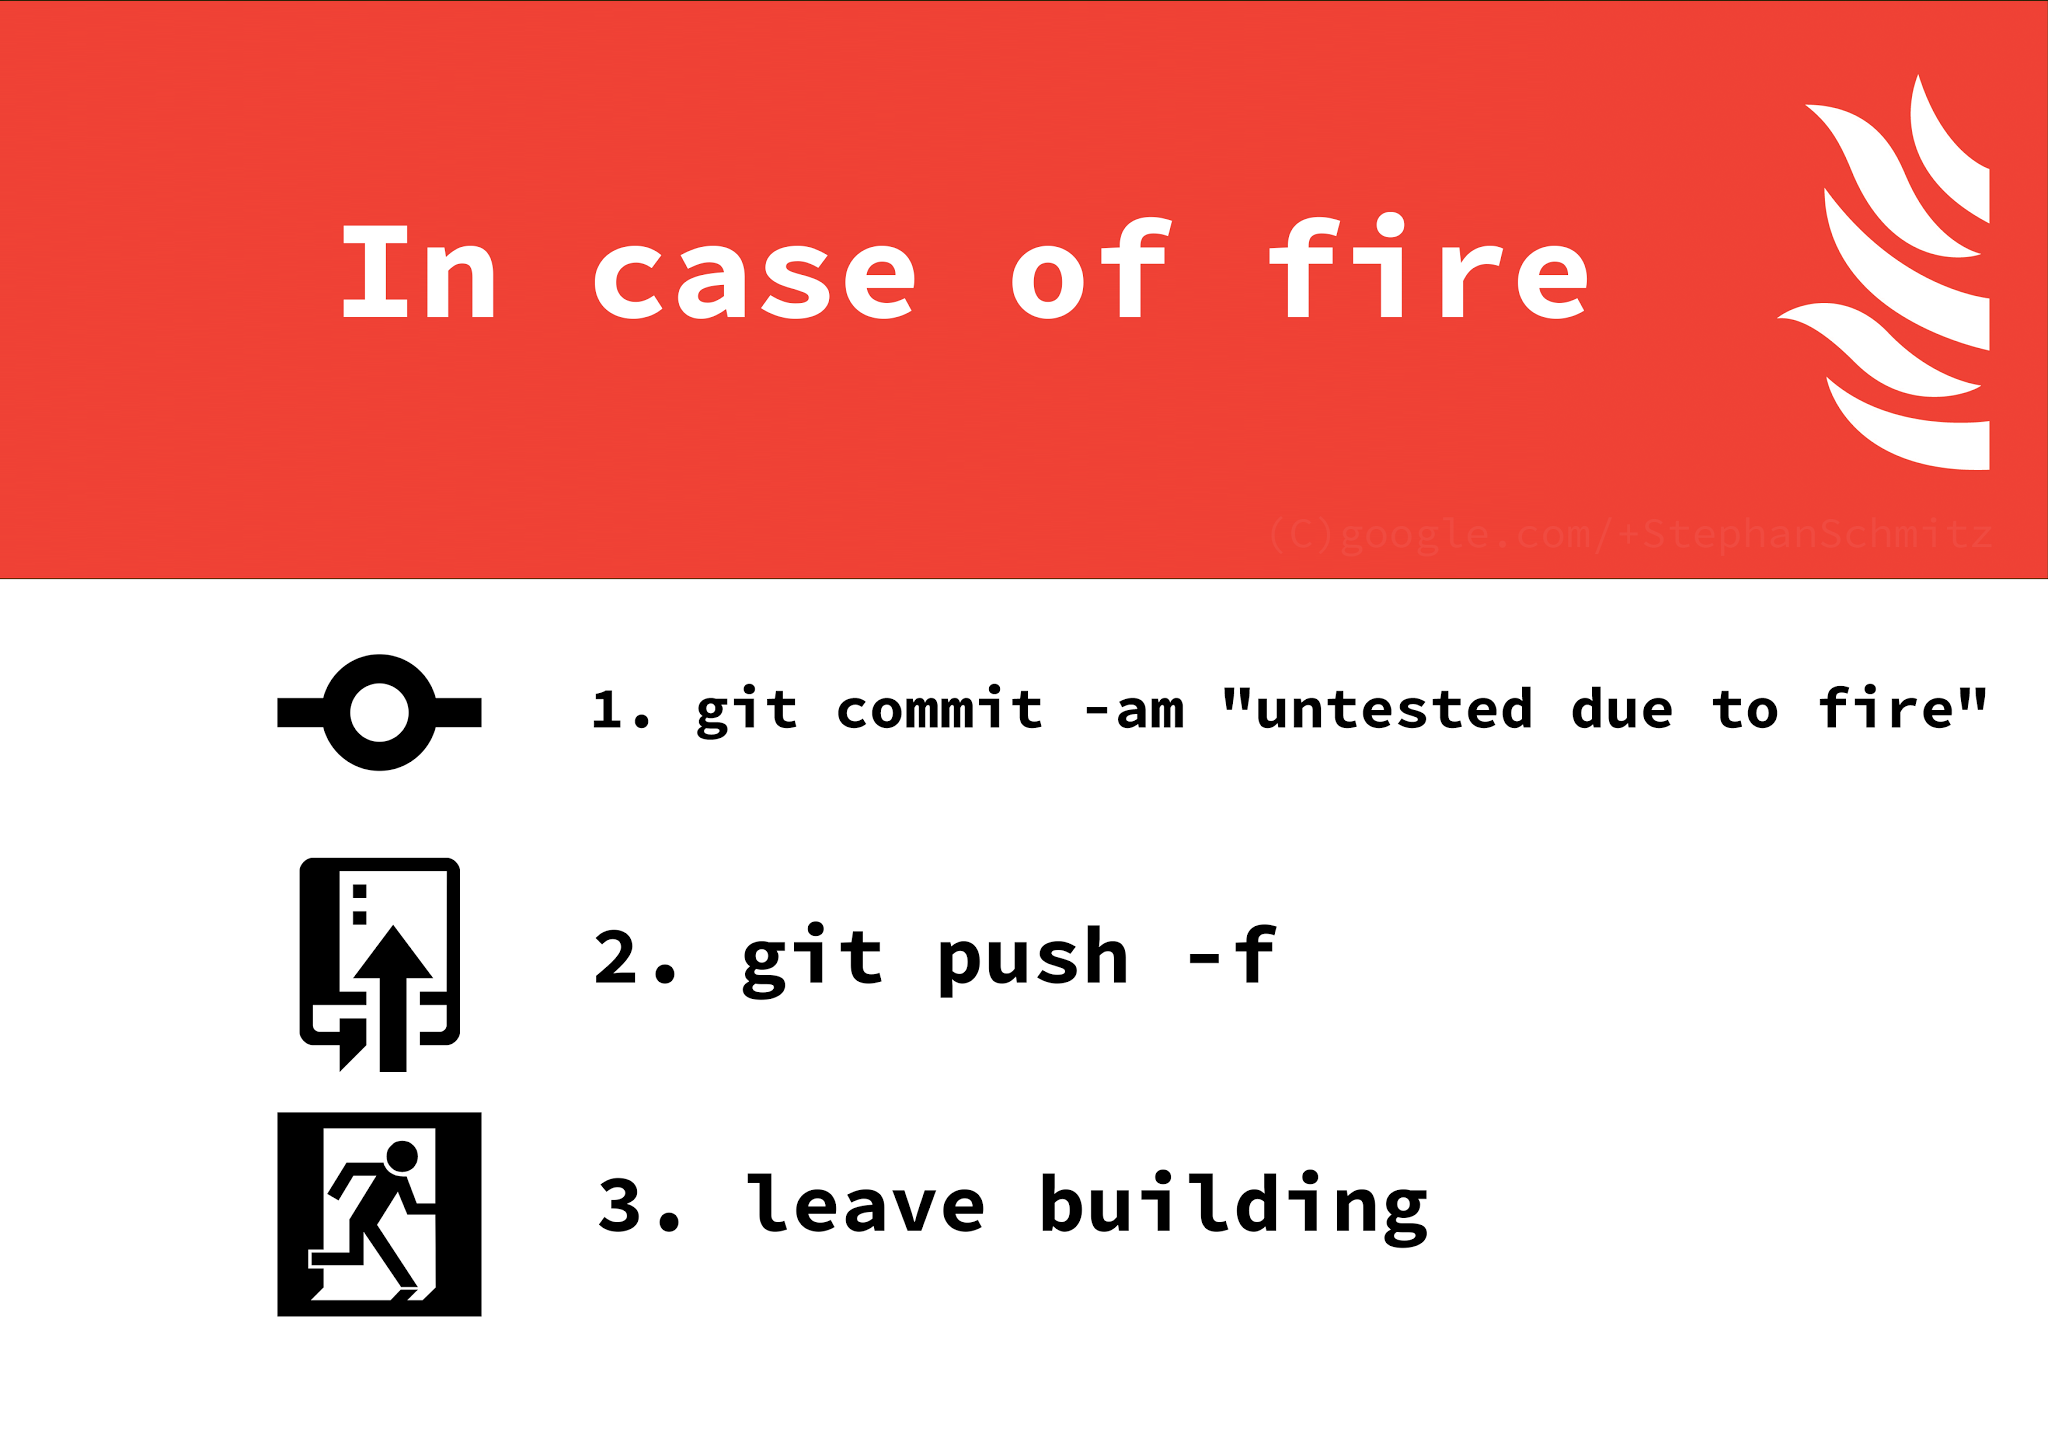
\includegraphics[width=0.7\linewidth]{Incaseoffire}
  \begin{itemize}
    \item Everything we will work on today, will be helpful if you work solo.
    \item These things will become really useful once you work with multiple people.
    \item The most useful tip I can give you is: \pause Consistency \& Discipline.
    \item We are going to talk about Workflows at the end of the day.
  \end{itemize}
\end{frame}
\begin{frame}[fragile]{Interlude: .gitconfig}
  The file \emph{.gitconfig} can be used to set default options per user or per project. The user files is in \emph{~/.gitconfig}. Each option can also be set with git \textbf{config}.
  \begin{lstlisting}
  [user]
    email = v.churavy@gmail.com
    name  = Valentin Churavy
  [github]
    user = vchuravy
  [push]
    default = simple
  [rerere]
    enabled = true
  \end{lstlisting}
\end{frame}
\subsection{Remotes}
\begin{frame}[fragile]
  Yesterday we introduced \textbf{Github}. Github is a service that offers you a solution to remotely store your repositories. 
  Git is \emph{Distributed} Version Control System (DVCS). Every copy of your repository, may it be remote or local, is independent of each other. There is no central master repository. 

  In order to synchronize these distributed copies we introduce the concept of a remote.
\pause
  \begin{block}{}
    git \textbf{remote}
  \end{block}
\pause
  There can be as many remotes as you want each with different names. When you clone a repository there will be one default remote called \textbf{origin}.
\end{frame}
\subsection{Branches}
\begin{frame}[fragile]
  Since there git is decentralized there is no one state of the repository that is correct. No manage this complexity git has the notion of a branch. Branches are parallel timelines and they lightweight, so branch often and branch early.
  \begin{block}{}
    \begin{itemize}
      \item git \textbf{branch}  Manages branches. 
      \item git \textbf{checkout} Switch between branches.
      \item git \textbf{cherry-pick} Moving commits between branches.
    \end{itemize}
  \end{block}
  Most repositories have a default branch called \textbf{master}. Branches are just names for points in the history.
  Once we start working with branches we have to ask ourselves how are we going to join them back up? We can do this by performing a merge.

  You can also associate a local branch with a remote branch by setting it as upstream. git push \textbf{-u}.
\end{frame}
\subsection{Merging}
\begin{frame}[fragile]
Merging is the act of joining two branches together or to join two different branches. You will always merge \emph{from} a branch/remote into a branch.
  \begin{block}{}
    \begin{itemize}
      \item git \textbf{fetch}  Get remote changes
      \item git \textbf{merge}  Merge changes (ff by default)
      \item git \textbf{add}    Resolve merge-conflict
    \end{itemize}

    Options for merge:
    \begin{description}
      \item[--no-commit] Performs the merge, but doesn't commit yet. Giving you the change to edit the merge commit.
      \item[--ff-only]   Aborts when we can't perform a fast-forward merge.
      \item[--abort]     Abort the current conflict-resolution and reset to previous state.
    \end{description}
  \end{block}

  You can visualize your history in many different ways, but the best way on the command line is.\\
  git log \textbf{--graph --pretty --oneline}
\end{frame}
\subsection{Rebasing and Rewriting history}
\begin{frame}[fragile]
  Rebases are a way to create fast-forward merges, by altering \emph{history}. Each branch has a root commit from which it diverged from the original commit. By rebasing we change this root. This has a couple of side effects. 
  \begin{itemize}
    \item Linear commit history.
    \item No merge commits within a branch.
    \item commit-ids change.
  \end{itemize}

  \begin{block}{}
    \begin{itemize}
      \item git \textbf{pull --ff-only} Don't merge if there are conflict with the remote
      \item git \textbf{rebase} Perform a rebase
      \item git \textbf{rebase -i} Perform a interactive rebase
      \item git \textbf{push -f} Force push your changes
      \item git \textbf{pull --rebase} Perform a pull with a rebase
    \end{itemize}
  \end{block}
\end{frame}
\begin{frame}[allowframebreaks]{Secrets!}
  \begin{block}{Autosquash}
    \begin{itemize}
      \item git config rebase.autosquash true
      \item git commit \textbf{--squash=}\emph{some-hash}
      \item git commit \textbf{--fixup=}\emph{some-hash}
     \end{itemize}
     Autosquash will reorder the commits apropriatly before you perform a git \textbf{rebase -i}.
  \end{block}
  \begin{block}{Bisect}
    You have a new test case that produces wrong results in your software. Question! When did the error first appear? Git bisect is here to help, by performing a binary search through history to find the last good commit (or the first bad commit).

    This is the reason, why every commit should be functional!.
  \end{block}
  \framebreak
  \begin{block}{Stash}
    When you are moving between branches you sometines want to keep your non-commited changes associated with the branch you where doing them one.
    \begin{itemize}
      \item git \textbf{stash}
      \item git \textbf{stash pop}
    \end{itemize}
  \end{block}
\end{frame}
\section{Workflow}
\begin{frame}[fragile]{Workflows}
  \centering
  Storytelling from the battlefields.
\end{frame}
\subsection{Documentation and other helpful material}
\begin{frame}{Documentation}
  \begin{itemize}
    \item The Git book: \url{https://git-scm.com/book}
    \item The Git help/man pages: git \textbf{help} or git \emph{command} --help
    \item Caching your password: \url{https://help.github.com/articles/caching-your-github-password-in-git/}
    \item SSH-keys: \url{https://help.github.com/categories/ssh/} 
  \end{itemize}
\end{frame}
\end{document}
